% Format teze zasnovan je na paketu memoir
% http://tug.ctan.org/macros/latex/contrib/memoir/memman.pdf ili
% http://texdoc.net/texmf-dist/doc/latex/memoir/memman.pdf
% 
% Prilikom zadavanja klase memoir, navedenim opcijama se podešava 
% veličina slova (12pt) i jednostrano štampanje (oneside).
% Ove parametre možete menjati samo ako pravite nezvanične verzije
% mastera za privatnu upotrebu (na primer, u b5 varijanti ima smisla 
% smanjiti 
\documentclass[12pt,oneside]{memoir} 

% Paket koji definiše sve specifičnosti master rada Matematičkog fakulteta
\usepackage[latinica]{matfmaster} 
%
% Podrazumevano pismo je ćirilica.
%   Ako koristite pdflatex, a ne xetex, sav latinički tekst na srpskom jeziku
%   treba biti okružen sa \lat{...} ili \begin{latinica}...\end{latinica}.
%
% Opicija [latinica]:
%   ako želite da pišete latiniciom, dodajte opciju "latinica" tj.
%   prethodni paket uključite pomoću: \usepackage[latinica]{matfmaster}.
%   Ako koristite pdflatex, a ne xetex, sav ćirilički tekst treba biti
%   okružen sa \cir{...} ili \begin{cirilica}...\end{cirilica}.
%
% Opcija [biblatex]:
%   ako želite da koristite reference na više jezika i umesto paketa
%   bibtex da koristite BibLaTeX/Biber, dodajte opciju "biblatex" tj.
%   prethodni paket uključite pomoću: \usepackage[biblatex]{matfmaster}
%
% Opcija [b5paper]:
%   ako želite da napravite verziju teze u manjem (b5) formatu, navedite
%   opciju "b5paper", tj. prethodni paket uključite pomoću: 
%   \usepackage[b5paper]{matfmaster}. Tada ima smisla razmisliti o promeni
%   veličine slova (izmenom opcije 12pt na 11pt u \documentclass{memoir}).
%
% Naravno, opcije je moguće kombinovati.
% Npr. \usepackage[b5paper,biblatex]{matfmaster}

% Pomoćni paket koji generiše nasumičan tekst u kojem se javljaju sva slova
% azbuke (nema potrebe koristiti ovo u pravim disertacijama)
\usepackage[latinica]{pangrami}
\usepackage{subfig}

% Datoteka sa literaturom u BibTex tj. BibLaTeX/Biber formatu
\bib{matfmaster-primer}

% Ime kandidata na srpskom jeziku (u odabranom pismu)
\autor{Lazar Čeliković}
% Naslov teze na srpskom jeziku (u odabranom pismu)
\naslov{Upravljanje razvojem mobilnih aplikacija sa fokusom na performanse i kvalitet}
% Godina u kojoj je teza predana komisiji
\godina{2024}
% Ime i afilijacija mentora (u odabranom pismu)
\mentor{dr Vladimir \textsc{Filipović}, redovan profesor\\ Univerzitet u Beogradu, Matematički fakultet}
% Ime i afilijacija prvog člana komisije (u odabranom pismu)
\komisijaA{dr Aleksandar \textsc{Kartelj}, vanredni profesor\\ Univerzitet u Beogradu, Matematički fakultet}
% Ime i afilijacija drugog člana komisije (u odabranom pismu)
\komisijaB{dr Staša \textsc{Vujučić Stanković}, docent\\ Univerzitet u Beogradu, Matematički fakultet}
% Ime i afilijacija trećeg člana komisije (opciono)
% \komisijaC{}
% Ime i afilijacija četvrtog člana komisije (opciono)
% \komisijaD{}
% Datum odbrane (odkomentarisati narednu liniju i upisati datum odbrane ako je poznat)
% \datumodbrane{}

% Apstrakt na srpskom jeziku (u odabranom pismu)
\apstr{%
Mobilne aplikacije i aplikacije generalno često se razvijaju sa primarnim ciljem da se pokrije što je moguće više funkcionalnosti, dok se koncepti kao što su performanse zanemaruju dok problem ne postane evidentan. U ovom radu se razmatra pristup koji ove koncepte stavlja u središte i implementira ih na samom početku razvojnog ciklusa. Rad prikazuje kako postavljanje sistema za merenje performansi, poslovnih metrika i analizu grešaka olakšava dalji razvoj u kasnijim stadijumima projekta. Rešenje koje ćemo analizirati razvijeno je uz pomoć razvojnog okruženja ReactNative uz podršku RTKQ biblioteke sa menadžovanje stanja podataka. Rad prikazuje detalje implementacije ovih sistema kao i benefite koje dobijamo korišćenjem istih. Pomenuti koncepti biće prikazani i analizirani na primeru mobilne aplikacije za vremensku prognozu.
}

% Ključne reči na srpskom jeziku (u odabranom pismu)
\kljucnereci{mobilna aplikacija, performanse, dogadjaji, računarstvo, programiranje}

\begin{document}
% ==============================================================================
% Uvodni deo teze
\frontmatter
% ==============================================================================
% Naslovna strana
\naslovna
% Strana sa podacima o mentoru i članovima komisije
\komisija
% Strana sa posvetom (u odabranom pismu)
% Strana sa podacima o disertaciji na srpskom jeziku
\apstrakt
% Sadržaj teze
\tableofcontents*

% ==============================================================================
% Glavni deo teze
\mainmatter
% ==============================================================================

% ------------------------------------------------------------------------------
\chapter{Uvod}
% ------------------------------------------------------------------------------
\pangrami

\section{Primeri korišćenja klasičnih \LaTeX{} elemenata}
% Primeri citiranja
Ovo je rečenica u kojoj se javlja citat \cite{PetrovicMikic2015}.
Još jedan citat \cite{GuSh:243}.
% Primeri navodnika
Isprobavamo navodnike: "Rekao je da mu se javimo sutra".
% Primer referisanja na tabelu (koja se javlja kasnije)
U tabeli \ref{tbl:rezultati} koja sledi prikazani su rezultati eksperimenta.
% Primer kraćeg ćiriličkog teksta
{\cir Ово је пример ћириличког текста који се јавља у латиничком документу.}
U ovoj rečenici se javlja jedna reč na {\cir ћирилици}.
% Primer korišćenja fusnota
Iza ove rečenice sledi fusnota.\footnote{Ovo je fusnota.}

% Primer dužeg ćirličkog teksta
\begin{cirilica}
  Ово је мало дужи блок текста исписан ћириличким писмом у оквиру
  латиничког документа. Фијуче ветар у шибљу, леди пасаже и куће иза
  њих и гунђа у оџацима.
\end{cirilica}

% Primer korišćenja tabele
\begin{table}
\centering
\caption{Rezultati}
\label{tbl:rezultati}
\begin{tabular}{c>{\centering}p{2cm}c}
\toprule
1 & 2 & 3\\\midrule
4 & 5 & 6\\\cmidrule(rl){1-2}
7 & 8 & 8\\
\bottomrule
\end{tabular}
\end{table}

% Primer korišćenja slike
\begin{figure}[!ht]
  \centering
  \label{fig:grafikon}
  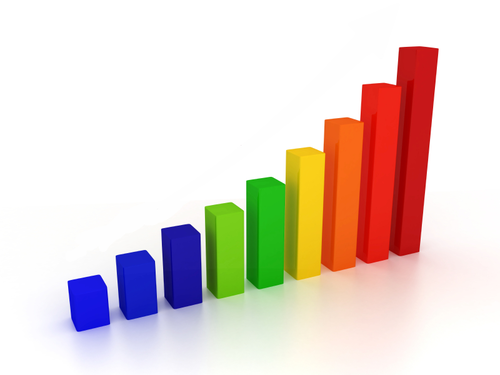
\includegraphics[width=0.5\textwidth]{graph.png}
  \caption{Grafikon}
\end{figure}


% Primer jednostavnije matematičke formule
Evo i jedan primer matematičke formule: $e^{i\pi} + 1 = 0$. 
% Primer referisanja na sliku
Na slici \ref{fig:grafikon} prikazan je jedan grafikon.

% primer kompleksnije matematičke formule
$$
\int_a^b f(x)\ \mathrm{d}x \ =_{def}\ \lim_{\max{\Delta x_k \rightarrow 0}} \sum_{k=1}^n f(x_k^*)\Delta x_k
$$

% primer referisanja na poglavlja i strane poglavlja
Više detalja biće dato u glavi \ref{chp:razrada} na strani \pageref{chp:razrada}.

% primer liste
Možemo praviti i nabrajanja:
\begin{enumerate}
\item Analiza 1
\item Linearna algebra
\item Analitička geometrija
\item Osnovi programiranja
\end{enumerate}

\pangrami

% ------------------------------------------------------------------------------
\chapter{Pregled tehnologija za razvoj mobilnih aplikacija}
\label{chp:pregledTehnologijaZaRazvojMobilnihAplikacija}

% ------------------------------------------------------------------------------
Mobilne aplikacije su doživele neverovatnu evoluciju od svog početka. Svedoci smo kako su one iz jednostavnih alata za komunikaciju ili zabavu prerastle u složene sisteme koji nam pomažu u svakodnevnom životu. Danas, aplikacije nisu samo način da ostanemo povezani s drugima, već i sredstvo za upravljanje finansijama, učenje novih veština, pa čak i za praćenje zdravlja i fitnessa. Razvoj tehnologija poput veštačke inteligencije i mašinskog učenja dodatno je unapredio funkcionalnost i intuitivnost aplikacija, pružajući korisnicima personalizovano iskustvo koje je prethodnih godina bilo nezamislivo. Ovaj napredak ne samo da je promenio način na koji interagujemo sa našim uređajima, već je i potpuno preoblikovao digitalni pejzaž, otvarajući nove mogućnosti za razvoj i inovacije u budućnosti. Ovaj napredak mobilnih aplikacija pratio je i razvoj tehnologija koje se koriste u izradi istih. Kroz vreme, došli smo do većeg broja tipova mobilnih aplikacija kao i do velikog broja radnih okvira koji nam omogućavaju lakši razvoj i održavanje aplikacija na kojima radimo.

\section{Tipovi mobilnih aplikacija}

Mobilne aplikacije mogu se kategorisati u nekoliko osnovnih tipova, svaki sa svojim specifičnim funkcijama i ciljevima. Delimo ih na nativne aplikacije(eng. native mobile applications), veb aplikacije (eng. web mobile applications), hibridne mobilne aplikacije i progrsivne veb alikacije (eng. progressive web applications - (PWA)). Svaki od ovih tipova ima svoje prednosti i mane, te izbor tipa aplikacije zavisi od specifičnih potreba i ciljeva projekta. U nastavku rada ćemo analizirati svaku od pomenutih kategorija.

\subsection{Nativne mobilne aplikacije}

Nativne mobilne aplikacije (eng. native mobile applications) su programi razvijeni za specifičan operativni sistem, kao što je iOS ili Android, koristeći programerske jezike koji su specifični za svaku od platformi. Tako imamo Swift i Objective C za iOS ili Kotlin i Javu za Android. Ove aplikacije se instaliraju direktno na mobilni uređaj preko prodavnice aplikacija na uređaju i optimizovane su da pružaju maksimalnu efikasnost i iskoristivost hardverskih karakteristika uređaja. Prednsoti ovog tipa mobilnih aplikacija su:

\begin{itemize}
    \item Budući da je ovaj tip aplikacija optimizovan za specifičnu platformu, po pravilu se mogu izvući neuporedivo više performanse u poređenju sa ostalim tipovima.
    \item Fluidne animacije i intuitivan interfejs koji potiče od samog operativnog sistema rezultuju poboljšanim korisničkim iskustvom.
    \item Mogućnost pristupa punom setu hardverskih i softverskih funkcija samog uređaja kao što su kamera, GPS, senzori
    \item Nativne mobilne aplikacije se objavljuju na prodavnicama aplikacija kao sto su Play prodavnica (eng. Play Store) i App prodavnica (eng. App store). Tokom ovog procesa se vrši detaljno ispitivanje aplikacija i na ovaj način se povećava sigurnost.
\end{itemize}
Mane ovog tipa mobilnih aplikacija su:
\begin{itemize}
    \item Razvijanje posebne aplikacija za svaki operativni sistem povećava troškove kao i vreme koje je potrebno da se aplikacija pusti u korišćenje
    \item Različiti operativni sistemi često iziskuju različite programske jezike za razvoj, što može otežati pronalaženje razvojnih timova.
    \item Svaka promena ili ažuriranje aplikacija zahteva odvojeno slanje na odobrenje prodavnicu aplikacija za svaki operativni sistem. Ovaj proces je često vremenski zahtevan.
\end{itemize}

\begin{figure}[h]
    \centering
    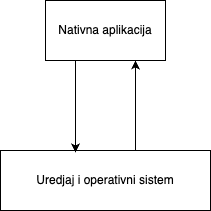
\includegraphics[scale=0.5]{docs/images/chapterTwo/nativnaAplikacija.png}
    \caption{Komunikacija nativne aplikacije i operativnog sistema}
    \label{fig:nativnaAplikacija}
\end{figure}

\subsection{Veb aplikacije}

Veb aplikacije (eng. web applications) su pristupačne preko internet pretraživača i ne zahtevaju preuzimanje i instalaciju na uređaj kao tradicionalne aplikacije. One su dizajnirane da budu kompatibilne sa različitim platformama i pružaju jedinstveno iskustvo korisnicima na različitim uređajima. One predstavljaju korisnu opciju za aplikacije koje zahtevaju brzu dostupnost i lako održavanje, ali kada je u pitanju duboka integracija sa uređajem i složene interakcije, ovaj tip aplikacije često zaostaje za mogućnostima koje pružaju nativne aplikacije. Prednosti veb mobilnih aplikacija:

\begin{itemize}
    \item Ovaj tip mobilnih aplikacija će raditi na bilo kom uređaju koji ima veb pretraživač. Ova osobina uklanja potrebu za posebnim verzijama za različite operativne sisteme.
    \item Ovaj tip mobilnih aplikacija razvija se samo jednom za sve platforme, čime se troškovi razvoja i ažuriranja značajno smanjuju u odnosu na nativne aplikacije.
    \item Korisnici veb aplikacija imaće pristup najnovijim izmenama onog momenta kada te izmene budu puštene na produkciju. Ovo znači da se uklanja potreba za preuzimanjem ažururanja, što znatno olakšava distribuciju i održavanje.
\end{itemize}
Mane ovog tipa mobilnih aplikacija su:
\begin{itemize}
    \item Veb mobilne aplikacije zavise od brzine i kvaliteta internet konekcije, a takođe ne mogu u potpunosti iskoristiti sve hardverske mogućnosti uređaja kao što to mogu nativne mobilne aplikacije.
    \item Korisnički interfejsi ovog tipa mobilnih aplikacija često su manje fluidni i intuitivni u odnosu na nativne mobilne aplikacije, što može uticati na ukupno korisničko iskustvo.
    \item Funkcionalnosti i performanse mogu varirati u zavisnosti od pretraživača koji korisnik upotrebljava, što može rezultovati u nekonzistentnosti u korisničkom iskustvu.
\end{itemize}

\begin{figure}[h]
    \centering
    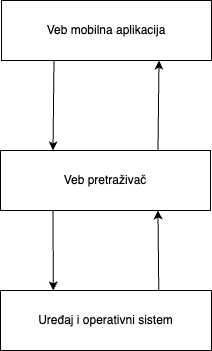
\includegraphics[scale=0.5]{docs/images/chapterTwo/vebMobilnaAplikacija.png}
    \caption{Komunikacija veb aplikacije i operativnog sistema}
    \label{fig:vebMobilnaAplikacija}
\end{figure}

\subsection{Progresivne veb mobilne aplikacije}

Progresivne veb aplikacije (eng. Progressive Web Applications (PWA)) su vrsta aplikacija koje kombinuju najbolje osobine tradicionalnih veb aplikacija i native mobilnih aplikacija. One se izvršavaju u veb pretraživaču, ali pružaju korisničko iskustvo koje je blisko iskustvu koje pružaju nativne mobilne aplikacije. PWA su dizajnirane da budu brze, pouzdane, čak i u uslovima loše internet konekcije. Osnovne prednosti ovog tipa aplikacija su:

\begin{itemize}
    \item Zahvaljujući servisnim radnicima (eng. service workers), progresivne veb aplikacije mogu raditi offline ili na slabim mrežnim konekcijama, pružajući osnovnu funkcionalnost kada nema internet konekcije.
    \item Korisnici mogu "instalirati" progresivne veb aplikacije na svoje uređaje, omogućavajući im da pristupe aplikaciji sa početnog ekrana, slično kao kod nativnih aplikacija.
    \item Progresivne veb aplikacije imaju podršku za notifikacija (eng. push notification), što omogućava bolje zadržavanje korisnika (eng. retention).
    \item Progresivne veb aplikacije zahtevaju HTTPS\footnote{eng. Hypertext transfer protocol secure} za pokretanje, što omogućava sigurniju razmenu podataka između korisnika i aplikacije.
\end{itemize}
Mane ovog tipa mobilnih aplikacija su:
\begin{itemize}
    \item Iako progresivne veb aplikacije imaju pristup nekim hardverskim funkcijama, one ne mogu potpuno iskoristiti sve kapacitete uređaja kao što to mogu nativne aplikacije.
    \item Ovaj tip aplikacija nije jednako podržan na svim platformama, s iOS uređajima koji imaju određena ograničenja u pogledu funkcionalnosti u odnosu na Android uređaje.
    \item Razvoj ovog tipa mobilnih aplikacija može biti složeniji od tradicionalnih veb aplikacija zbog potrebe za implementacijom servisnih radnika i upravljanjem keširanim podacima za offline rad.
\end{itemize}

U poređenju sa tradicionalnim web aplikacijama, PWA pružaju bolje korisničko iskustvo, veću pouzdanost i više funkcionalnosti koje su bliske native iskustvu, čineći ih izuzetno privlačnim izborom za razvoj aplikacija koje treba da budu efikasne i dostupne širom različitih platformi i uslova povezivanja.

\subsection{Hibridne mobilne aplikacije}

Hibridne mobilne aplikacije (eng. crossplatform mobile application) predstavljaju spoj nativnih i veb tehnologija, omogućavajući razvoj aplikacija koje se mogu instalirati na uređaj, ali se izvršavaju u veb kontejneru. Ove aplikacije koriste kombinaciju HTML, CSS, i JavaScript za izradu korisničkog interfejsa, dok istovremeno koriste mostove (eng. bridge) poput Cordova ili Ionic za pristup native funkcijama uređaja. Ovaj tip aplikacije biće implementiran u okviru ovog rada pa ćemo imati prilike detaljnije da se upoznamo sa karaktiristikama istih. Osnovne prednosti ovog tipa mobilnih aplikacija su:

\begin{itemize}
    \item Razvoj se vrši koristeći veb tehnologije koje su mnogim programerima već poznate, što smanjuje vreme i troškove razvoja.
    \item Jedan kod može se koristiti za više platformi (iOS, Android, Windows Phone), što dodatno smanjuje troškove i olakšava održavanje.
    \item Kroz različite biblioteke, hibridne mobilne aplikacije mogu koristiti hardver uređaja (kamere, GPS, senzore i druge funkcije).
\end{itemize}
Mane ovog tipa mobilnih aplikacija su:
\begin{itemize}
    \item Zbog dodatnog sloja apstrakcije i oslanjanja na veb tehnologije, performanse hibridnih aplikacija mogu biti lošije u odnosu na nativne aplikacije, posebno za zahtevne zadatke. Ovo je idealan razlog zbog koga bi trebalo razmotriti implementiranje sistema za praćenje performansi na početku razvoja aplikacije.
    \item Iako se ne trude da imitiraju izgled i osećaj nativnih aplikacija, hibridne mobilne aplikacije često ne mogu potpuno replicirati fludinost i odziv nativnog korisničkog interfejsa.
    \item Ovaj tip mobilnij aplikacija zavisi od platformi kao što su Cordova ili Ionic, što može dovesti do problema ako se ti alati ne ažuriraju redovno ili ne podržavaju najnovije verzije operativnih sistema.
\end{itemize}

\begin{figure}[h]
    \centering
    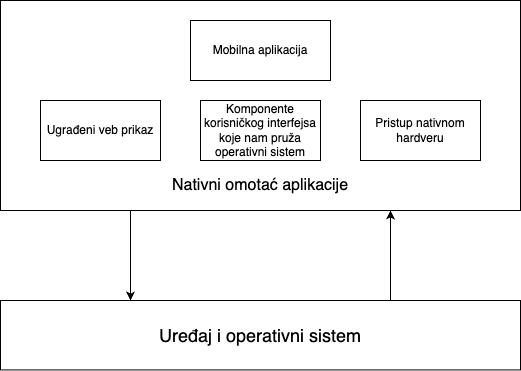
\includegraphics[scale=0.5]{docs/images/chapterTwo/hibridnaMobilnaAplikacija.png}
    \caption{Komunikacija hibridne mobilne aplikacije i operativnog sistema}
    \label{fig:hibridnaMobilnaAplikacija}
\end{figure}

\chapter{Osnove radnog okvira React Native}

React Native (eng. React Native) predstavlja JavaScript radni okvir (eng. framework) za kreiranje mobilnih aplikacija za iOS i Android operativne sisteme. Zasnovan je na React radnom okviru, sa izmenom da targetuje mobilne uređaje. Dakle, ovaj radni okvir omogućava nam da kreiramo mobilne aplikacije koje imaju nativni izgled kao i korisničko iskustvo, a sve to korišćenjem dobro poznatih veb tehnologija. React Native razvijen je 2015. godine od strane kompanije Meta Inc., ranije poznata kao Facebook Inc. Od tada, sam radni okvir se dosta izmenio i postao je jedan od najpopularnijih alata za ravoj mobilnih aplikacija.

\section{Kako React Native zapravo radi}

Osnovna ideja iza ovog radnog okvira jeste da kombinuje dve zasebne celine - JavaScript kod sa jedne i nativni kod sa druge strane (Java/Kotlin za Android i Ojective-C/Swift za iOS) i učini da njih dve međusobno sarađuju. Nativni kod će se izvršavati na samom uređaju, dok će za JavaScript kod biti neophodna virtuelna mašina. Ovo nam nije problematično na iOS uređajima iz razloga što oni poseduju ugrađeni JavaScript pokretač nazvan JavaScriptCore. Android uređaji nemaju ugrađen ovaj pokretač, međutim React Native se brine za to i on donosi isto za Android uređaje. Napomenućemo ovde da ovo rezultuje time da se veličina same aplikacije povećava za Android.

\subsection{Komunikacija između uređaja i JavaScript-a}

Kako se programski jezici koji se koriste na samim uređajima razlikuju od JavaScript programskog jezika neophodno je da se kreira neki protokol kako bi oni mogli međusobno da komuniciraju. Ovo se postiže preko formata koji obe strane razumeju, a to je JSON. Sva komunikacija između ovih delova sistema obavlja se preko mosta (eng. Bridge).

\subsection{Niti korišćene u React Native radnom okviru}

Kada korisnik pokrene React Native aplikaciju, sam uređaj će kreirati tri glavne niti i ostale ukoliko za istim postoji potreba. Niti koje će biti kreirane su Glavna nit (eng. Main Thread), JavaScript nit (eng. JavaScript thread) i nit u senci (eng. Shadow Thread).

\begin{itemize}
    \item Glavna nit (eng. Main Thread) - ova nit poznata je i kao nit korisničkog interfejsa. To je osnovna nit svaki iOS ili Android aplikacije i predstavlja glavnu nativnu nit na kojoj će se naša aplikacije izvršavati. Njena odgovornost jeste da obrađuje korisničke interakcije sa uređajem kao i da ažurira sam korisnički interfejs na ekranu uređaja. U React Native radnom okviru sve nativne komponente se renderuju na ovoj niti i iz ovog razloga je veoma bitno da se izbegavaju složene operacije na ovoj niti kako ne bi došlo do blokiranja korisničkog interfejsa i smanjenja performansi.
    \item JavaScript nit (eng. JavaScript Thread) - na ovoj niti će se izvršavati sav JavaScript i React kod naše aplikacije. Ona obrađuje logiku aplikacije, API pozive, vrši proračune i upravlja stanjem aplikacije. Ova nit je ključna za sve što nije povezano sa korisničkim interfejsom. Ova nit radi zasebno od glavne niti što nam omogućava da radimo kompleksna izračunavanja bez da blokiramo glavnu nit. 
    \item Nit u senci (eng. Shadow Thread) - ova nit poznata je jos i kao nit rasoreda (eng. Layout Thread) . Odgovornost ove niti jeste da preračunava pozicije elemenata i da generiše stablo za prikazivanje koje je kodirano u JavaScript niti. Kada se ovo izračunavanje završi ti podaci se šalju glavnoj niti koja vrši prikazivanje. Njena uloga jeste da oslobodi glavnu nit ovog posla, koji može biti veoma zahtevan. Ovaj pristup nam omogućava da imamo fluidno korisničko iskustvo.
\end{itemize}

\begin{figure}[h]
    \centering
    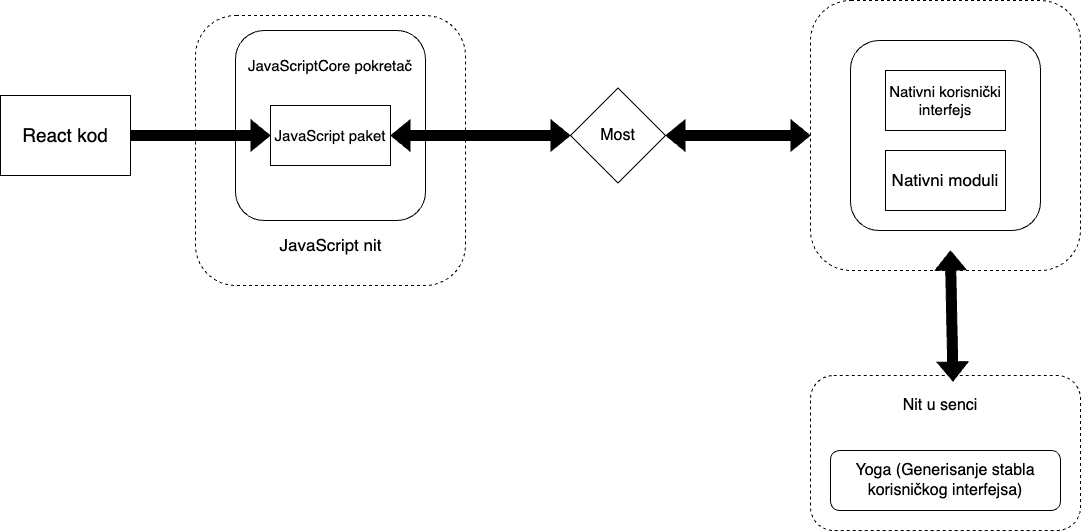
\includegraphics[scale=0.4]{docs/images/chapterThree/reactNativeArchitecture.png}
    \caption{Arhitektura React Native radnog okvira}
    \label{fig:reactNativeArchitecture}
\end{figure}

\section{Most u React Native radnom okviru}

U arhitekturi radnog okvira React Native, most (eng. bridge) igra ključnu ulogu u omogućavanju komunikacije između JavaScript niti i nativnih delova aplikacije koji se izvršavaju na glavnoj niti. Ovaj most funkcioniše kao posrednik koji prenosi informacije između dve sredine koje inače ne bi mogle direktno da komuniciraju zbog različitih programskih jezika (JavaScript sa jedne i Objective-C i Java sa druge strane). Komunikacija se obalja asinhronom razmenom JSON poruka izmedju ova dva okruženja. JavaScript kod se izvršava u svom okruženju, dok se nativne komponente upravljaju kroz specifične platforme kao što su iOS ili Android. Most omogućava asinhronu komunikaciju između ova dva okruženja prenošenjem poruka, što znači da informacije mogu preći iz jednog okruženja u drugo bez blokiranja glavne niti ili usporavanja aplikacije. Kada JavaScript kod zahteva pristup nativnim funkcionalnostima (kao što su pristup kameri ili GPS-u) ili kada treba da se ažurira korisnički interfejs, most prenosi ove zahteve iz JavaScript-a u nativni sistem, i obratno, prenosi odgovore nazad. Ovaj mehanizam omogućava React Native aplikacijama da koriste prednosti kako veb tehnologija, tako i nativnih performansi, iako ponekad može predstavljati usko grlo u performansama ako se prevelik broj zahteva mora preneti preko mosta.

\begin{figure}[h]
    \centering
    
\includegraphics[scale=0.5]{docs/images/chapterThree/reactNativeBridge.png}
    \caption{Funkcionisanje mosta}
    \label{fig:reactNativeBridge}
\end{figure}

\subsection{Primer rada mosta}

Sada ćemo proći kroz primer kako most izvodi komunikaciju između nativnog dela i JavaScript dela mobilne aplikacije.

\begin{enumerate}
    \item Okida se nativni događaj. Recimo da je u pitanju klik na dugme.
    \item Serijalizovana poruka šalje se sa nativne strane kroz most sa svim neophodnim podacima
    \item JavaScript prima poruku, deserijalizuje je i odlučuje šta je sledeći korak koji je potrebno preduzeti. U ovom slučaju to je akcija koja je pridružena dugmetu.
    \item Šalje se poruka sa JavaScript strane kroz most sa svim potrebnim informacijama vezanima za traženu akciju.
    \item Nativna strana prima poruku, deserijalizuje je i vrši ponovno renderovanje korisničkog interfejsa.
\end{enumerate}

\subsection{Nedostaci mosta}

Asinhrona priroda prenosa poruka između nativnog i JavaScript dela mobilne aplikacija dovodi do problema koji se manifestuju u ivičnim slučajevima. Na primer, pretpostavimo da imamo polje za unos teksta gde korisnik unosi broj kartice. Želimo da formatiramo taj unos tako što ćemo ubaciti prazan karakter posle svakog četvrtog karaktera u kartici. Ova logika biće implementirana na JavaScript strani. Problem koji se ovde uočava jeste taj da kada korisnik pritisne peti broj po redu nativna strana aplikacije to javlja JS strani. Broj se nadovezuje na prethodni broj kartice i to se javlja nativnoj strani koja će ovo prikazati. Ovo dovodi do toga da će prvo biti renderovan broj bez razmaka, a tek kasnije će se izvršiti formatiranje i preko mosta će biti poslata sledeća poruka koja će nativnoj strani reći da treba da renderuje i razmak. Naravno, ukoliko most nije previše opterećen u tom momentu korisnik ne bi mogao da primeti ovo. Međutim, u situaciji kada se ogroman broj operacija izvršava paralelno ovo je vrlo moguća situacija. Drugi problem koji možemo da primerimo jeste da se svaka poruka mora serijalizovati na jednoj i deserijalizovati na drugoj strani, što dovodi do povećane potrošnje resursa.

\subsection{Rešenja prethodno pomenutih problema}

React Native tim adresirao je prethodne probleme i pristupio kreiranju načina da se isti prevaziđu. Kao rezultat toga od verzije 0.68 u mogućnosti smo da koristimo skroz novu arhitekturu koja odbacuje mehanizam mosta i počinje da koristi JavaScript interfejs (eng. JavaScript Interface - JSI). JSI predstavlja sloj opšte upotrebe koji može biti ugrađen u bilo koji JS pokretač i pomoću njega možemo kreirati direktnu konekciju ka nativnim interfejsima. Ovaj napredak postignut je tako što su nativni Java ili Obj-C metodi izloženi JS-u preko objekta domaćina (eng. HostObject). JS će čuvati referencu na ovaj objekat i preko njega će pristupati nativnim interfejsima.

\chapter{Aplikacija za vremensku prognozu}

U poglavlju koje sledi u nastavku bliže ćemo se upoznati sa aplikacijom za vremensku prognozu koja će se koristiti za demonstraciju koncepata koje analiziramo u okviru ovog master rada, kao i sa ključnim tehnologijama korišćenim u izradi iste.

\section{Korisnički interfejs aplikacije}

U ovoj sekciji ćemo se detaljno upoznati sa korisničkim interfejsom aplikacije. Kada razmislimo malo o tome, korisnički interfejs jeste jedan od najznačajnijih delova same aplikacije. Vrlo je bitno da isti bude jednostavan za korišćenje, intuitivan, ali i prijatan za oko, odnosno lepo dizajniran. Sve ove osobine korisničkog interfejsa osiguraće nam da naši korisnici koriste aplikaciju iznova. U ovom konkretnom slučaju imamo aplikaciju koja se sastoji od dva ekrana. Prvi ekran jeste taj na kome se pokazuju svi parametri vremenske prognoze, dok je drugi ekran odgovoran za pretragu destinacije za koju nam je potrebna vremenska prognoza.

\begin{figure}%
    \centering
    \subfloat[\centering Glavni ekran aplikacije]{{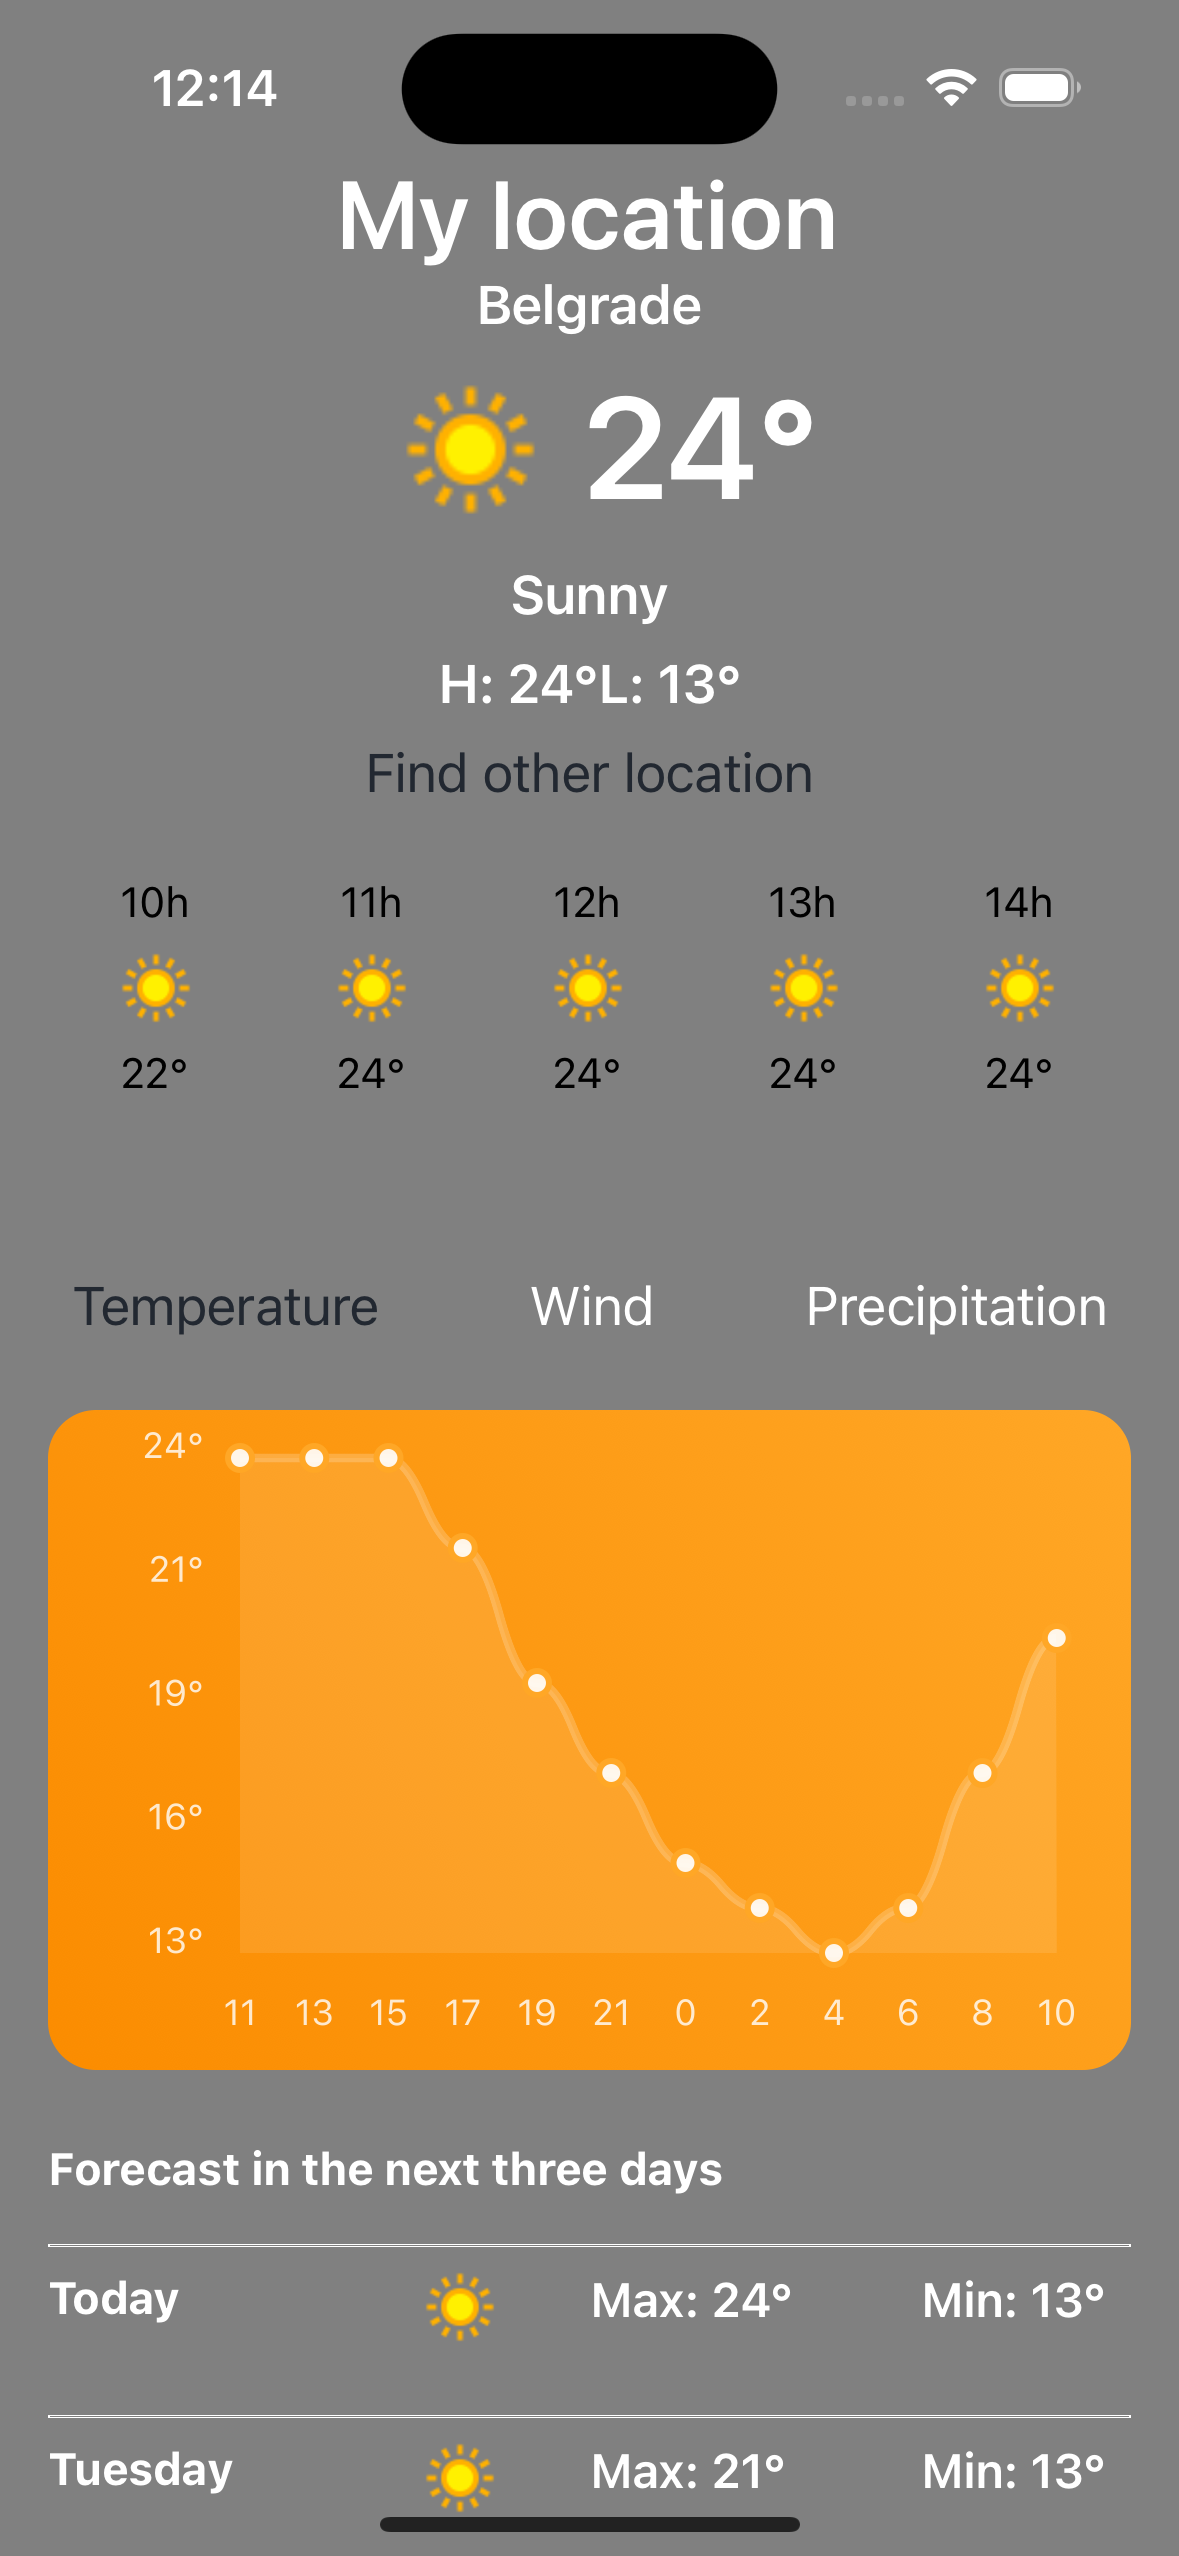
\includegraphics[width=5cm]{docs/images/chapterFour/mainScreen.png} }}%
    \qquad
    \subfloat[\centering Ekran za pretragu destinacije]{{
\includegraphics[width=5cm]{docs/images/chapterFour/searchScreen.png} }}%
    \label{fig:example}%
\end{figure}

\newpage
\subsection{Ekran za vremensku prognozu}

Glavni ekran aplikacije predstavlja ekran sa svim parametrima vremenske prognoze. Sastoji se od pet sekcija. U nastavku ćemo analizirati svaku.

\begin{enumerate}
    \item Prva sekcija predstavlja podatke o trenutnoj lokaciji i temperaturi. Takođe, tu imamo podatke u maksimalnoj i minimalnoj dnevnoj temperaturi kao i o tome kakvo je vreme napolju.
    \item Nakon ovoga nalazi se dugme koje nas navigira na ekran za pretragu drugih destinacija na kojima želimo da vidimo vremensku prognozu.
    \item Zatim, imamo listu koja prikazuje temperature na datoj lokaciji u naredna dvadeset četiri časa. U pitanju je horizontalna, skrolabilna optimizovana lista. U kasnijim poglavljima ćemo dodatno govoriti o ovim optimizacijama.
    \item Ispod se nalazi komponenta koja prikazuje grafike kretanja određenih parametara kroz vreme. Posmatra se period od dvadeset četiri časa i korisnik je u mogućnosti da selektuje parametar koji ga interesuje.
    \item Na kraju, imamo sekciju koja predstavlja vremensku prognozu za naredne dane. Realizovana je takođe kao optimizovana lista, sa izmenom da je sada vertikalna lista u pitanju.
\end{enumerate}

\subsection{Ekran za pretragu destinacije}

Drugi ekran u našoj aplikaciji služi za pretragu destinacije na kojoj korisnik želi da pogleda vremensku prognozu. Što se tiče korisničkog interfejsa na ovom ekranu, možemo videti da je malo jednostavniji u odnosu na prvi ekran. Kao što vidimo sa slike, izdvajaju se dve glavne celine.

\begin{enumerate}
    \item Na samom vrhu ekrana nalazi se navigacijsko zaglavlje koje je izmenjeno tako da bude komponenta za unos teksta. Ovde korisnik preko tastature unosi željenu lokaciju i preko aplikacijskog programskog interfejsa (eng. Application Programming Interface - API) dohvatamo niz lokacija za uneti teskt.
    \item Uloga druge sekcije jeste da se prikažu podaci koje nam je API vratio. Realizovana je takođe kao optimizovana lista.
\end{enumerate}

\subsection{WeatherAPI}

U svrhe dohvatanja podataka potrebnih za izradu ove aplikacije korišćen je WeatherAPI. U pitanju je API koji nam daje nekoliko krajnjih tačaka (eng. endpoint). Konkretno, mi smo koristili dva. 

\begin{enumerate}
    \item Forecast API - ovaj API nam služi za dohvatanje podataka o vremenskoj prognozi. Odgovor servera sastoji se iz tri celine. Podaci o trenutnoj lokaciji, podaci o trenutnom vremenu i podaci o vremenskoj prognozi za naredne dane.
    \item Search API - uloga ove krajnje tačke jeste da nam vrati sve lokacije koje počinju nekim prefiksom koji je korisnik uneo. 
\end{enumerate}

\newpage

\begin{figure}[h]
    \centering
    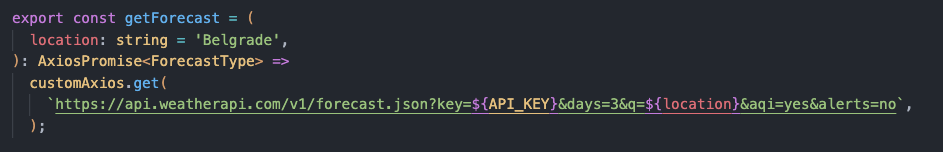
\includegraphics[scale=0.5]{docs/images/chapterFour/forecastAPI.png}
    \caption{API za vremensku prognozu}
    \label{fig:forecastAPI}
\end{figure}

\chapter{Sistem za merenje performansi aplikacije}

U savremenom razvoju softvera, efikasnost i performanse jedan su od ključnih aspekata za uspeh na tržištu. Uspeh naše aplikacije direktno zavisi od zadovoljstva korisnika, a to zadovoljstvo nemoguće je postići ukoliko aplikacija nije performantna. Ovo jeste razlog za razmatranje i uvođenje sistema za merenje performansi koji nam može pružiti jasnu sliku o ponašanju aplikacije u različitim uslovima. 
\newline
U ovom poglavlju upoznaćemo se sa različitim sistemima za merenje performansi i detaljnije se zadržati na sistemu Sentry. Proćićemo neophodne korake za integraciju ovog sistema u našu aplikaciju, a zatim se upoznati sa svime što nam isti pruža. Takođe, bavićemo se optimizovanim listama kao jedinom od ključnih koncepata u razvoju mobilne aplikacije.

\section{Alati za merenje performansi}

Kao što smo prethodno naveli, postoji veliki broj dostupnih platformi koje nam omogućavaju da integrišemo merenje performansi u našu aplikaciju. Pre nego što se upustimo u taj korak neophodno je upoznati se sa svima i odlučiti koji od tih alata najviše odgovara našim potrebama. U nastavku ove sekcije upoznaćemo se sa nekoliko najpopularnijih alata.

\subsection{React Native Performance Monitor}

React Native Performance Monitor je ugrađeni alat koji dolazi u okviru React native radnog okvira. On nam pruža osnovne informacije o performansama koje uključuju:

\begin{enumerate}
    \item Praćenje broja frejmova u sekundi (eng. Frame Per Second - FPS) - možemo pratiti dva seta FPS metrika. Jedan jeste za JavaScript nit, dok je drugi za glavnu, odnosno nit korisničkog interfejsa. Ovo nam omogućava da u realnom vremenu pratimo ove metrike i identifikujemo zbog čega dolazi do para performansi u nekom određenom momentu. Optimalno je da obe ove metrike budu blizu 60 FPS.
    \item Upotreba memorije - druga metrika koju možemo pratiti jeste količina radne memorije koju aplikacija koristi. Ovo nam je idealno za pronalaženje curenja memorije ili drugih problema vezanih za upravljanje memorijom.
\end{enumerate}

Iako je React Native Performance Monitor koristan za osnovno praćenje performansi aplikacije, on nije dovoljno detaljan i ne pruža nam dublji uvid u performanse aplikacije.

% ------------------------------------------------------------------------------
\chapter{Zaključak}
% ------------------------------------------------------------------------------
\pangrami

\pangrami

% ------------------------------------------------------------------------------
% Literatura
% ------------------------------------------------------------------------------
\literatura

% ==============================================================================
% Završni deo teze i prilozi
\backmatter
% ==============================================================================

% ------------------------------------------------------------------------------
% Biografija kandidata
\begin{biografija}
  \textbf{Vuk Stefanović Karadžić} (\emph{Tršić,
    26. oktobar/6. novembar 1787. — Beč, 7. februar 1864.}) bio je
  srpski filolog, reformator srpskog jezika, sakupljač narodnih
  umotvorina i pisac prvog rečnika srpskog jezika.  Vuk je
  najznačajnija ličnost srpske književnosti prve polovine XIX
  veka. Stekao je i nekoliko počasnih mastera.  Učestvovao je u
  Prvom srpskom ustanku kao pisar i činovnik u Negotinskoj krajini, a
  nakon sloma ustanka preselio se u Beč, 1813. godine. Tu je upoznao
  Jerneja Kopitara, cenzora slovenskih knjiga, na čiji je podsticaj
  krenuo u prikupljanje srpskih narodnih pesama, reformu ćirilice i
  borbu za uvođenje narodnog jezika u srpsku književnost. Vukovim
  reformama u srpski jezik je uveden fonetski pravopis, a srpski jezik
  je potisnuo slavenosrpski jezik koji je u to vreme bio jezik
  obrazovanih ljudi. Tako se kao najvažnije godine Vukove reforme
  ističu 1818., 1836., 1839., 1847. i 1852.
\end{biografija}
% ------------------------------------------------------------------------------

\end{document}
